% !TEX root = ../report_template.tex
\section{Dataset overview}\label{sec:data}
% 4 points. The task sheet's points are guidelines, not a checklist.

\subsection{Exploration of synthetic and real tables}\label{sec:exploration}
% What kinds of tables does the prior generate (sizes, feature types, number
% of classes, targets)? What do the benchmark datasets (\tabpfnval{},
% \citealt{hollmann2025tabpfn}) look like? Show examples made with show().

\paragraph{Synthetic tables from the prior.}
The model is pretrained only on synthetic tables, drawn from a \emph{prior}:
a program that defines a distribution over datasets
\citep{muller2022pfn,qu2026tabiclv2}. We use the prior of \nanotabicl{}
\citep{nanotabicl}, a slightly simplified version of the \tabicl{} prior
(\citealt{qu2026tabiclv2}, Sec.~5 and App.~E). For each table it draws a
random graph of 2 to 32 nodes; each node applies one of eight random function
types (e.g.\ neural networks, tree ensembles, Gaussian processes) to its
parents, or holds random points if it has none. Features and label are read
from random nodes; categorical columns and the label come from node values by
nearest-center assignment or by sampling from a softmax. A table whose label a
small ExtraTrees model cannot predict better than a constant is drawn again
(App.~E.14), so every table has some signal.

With our settings, a table has 320 to 2,048 training rows (80\% of 400 to
2,560 rows, log-uniform), 2 to 100 features (log-uniform) and one
classification label whose number of classes is drawn uniformly from 2 to 10.
The share of categorical columns is drawn from $[-0.5, 1.2]$ and
clipped to $[0, 1]$: 41\% on average, and at least 29\% of the tables have
none. A categorical column has 2 to 100 categories, given to the model as
integer codes. For evaluation we use 1,600 saved prior tables.

\paragraph{Real tables.}
The real benchmark, \tabpfnval{}, consists of the 57 classification
datasets that \citet{hollmann2025tabpfn} used to develop \tabpfn{}
(Supplementary Table~5). That list already leaves out datasets with more than
500 features or more than 10 classes. \tabicl{} uses these datasets for its
ablations; the paper speaks of 60 (\citealt{qu2026tabiclv2}, Fig.~10), but the
supplementary table lists 57. The datasets come from
many domains, for example medicine (\dataset{heart-c}), credit
(\dataset{heloc}) and criminal justice (\dataset{compas-two-years}). They have
2 to 299 features (median 16) and 42 to 2,048 training rows (median 763);
32 of 57 are binary. In 32 datasets at least one column is stored as text,
which we count as categorical (311 of 1,826 columns); numerically coded
categories are not counted. 12 datasets have missing values.

\paragraph{Examples.}
\Cref{fig:example_tables}, made with our \emph{show} function, shows three
prior and three real tables, each projected onto its first two principal
components. The prior tables differ a lot: in prior table~1 (middle) the
classes lie along a curve and are well separated, while the seven classes of
prior table~2 (right) overlap. The real tables show the same range: one
penguin species is clearly separate and the other two sit side by side, the
two classes of
\dataset{heart-statlog} overlap, and \dataset{breast-tissue} has only 85
training rows for six classes. A projection onto two axes hides the other
directions, so overlap here does not mean the classes cannot be separated.

\begin{figure}[t]
  \centering
  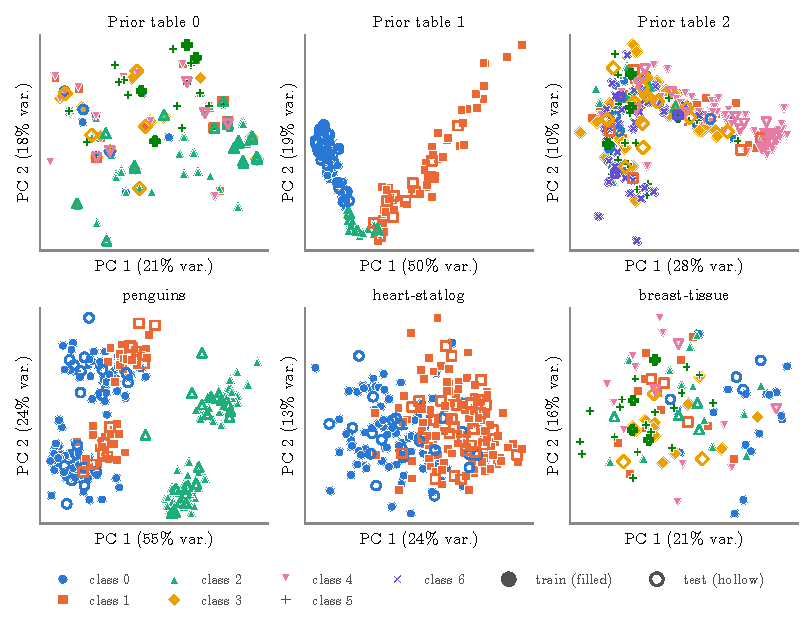
\includegraphics[width=\linewidth]{example_tables}
  \caption{Example tables. Top: the first three saved prior tables (not
    hand-picked). Bottom: three OpenML tables with 3, 2 and 6 classes. Each
    panel shows one table, projected onto the first two principal components
    of its standardized training rows. Filled markers are training rows, hollow markers are
    test rows, and each class has its own color and shape (at most 250 rows
    shown per table).}
  \label{fig:example_tables}
\end{figure}

\Cref{fig:table_shapes} compares the shapes of all tables. The prior covers
the features of the real tables up to 100, but three real datasets have more
(168, 260 and 299). The real tables are often smaller: 21 of 57 have fewer
than 320 training rows, the smallest size the model saw in training. And while
the prior's tables spread over 2 to 10 classes, more than half of the real
tables are binary. (Tables with many classes are a bit rarer in the prior than
drawn, because a class can end up with no training rows.)

\begin{figure}[t]
  \centering
  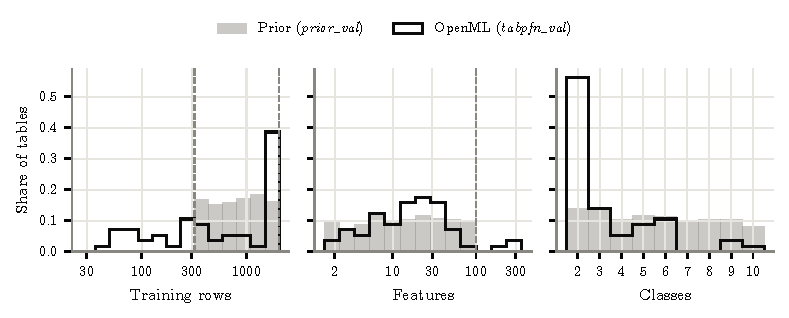
\includegraphics[width=\linewidth]{table_shapes}
  \caption{Share of tables per number of training rows, features and classes
    for the 1,600 saved prior tables and the 57 OpenML tables (split 0).
    Dashed lines: the range the prior was trained on (320 to 2,048 training
    rows, at most 100 features). 2,048 is also the cap on the OpenML training
    rows, so the 19 OpenML tables at the cap are larger datasets from which
    2,048 training rows were sampled.}
  \label{fig:table_shapes}
\end{figure}

\subsection{Data quality and splits}\label{sec:quality}
% Problems that could distort the evaluation: degenerate synthetic tables,
% duplicates between train and test rows, class imbalance, outliers.

\paragraph{Splits.}
For each OpenML dataset, 20\% of the rows (rounded) form the test set, and a
random sample of at most 2,048 of the other rows forms the training set; for
the 19 datasets with more than 2,560 rows, some rows are not used. The split
is stratified by class, and we use two splits with different random seeds, as
the paper does (\citealt{qu2026tabiclv2}, Fig.~10). Rows without a label are
dropped, which only happens in \dataset{Midwest\_Survey\_nominal} (284 of
2,778 rows). \dataset{birds} has 19 label columns, one per bird species; we
predict the most common species (Swainson's thrush) and drop the other label
columns from the features. Prior rows are generated in random order, so the
first 80\% of a table are a random training set. The 1,600 saved prior tables
use a different random seed than pretraining.

\paragraph{Checks.}
We checked every evaluation table for problems that could distort the
evaluation (\Cref{tab:quality}). The most common problem on the OpenML
datasets is test rows that also appear among the training rows: 22 of 57
datasets have them, 14\% of all OpenML test rows (prior: 497 of 1,600 tables,
20\%). This is not a mistake in the split. Tables with few discrete features
repeat rows naturally: \dataset{Titanic} has three features and only 14
distinct rows, so 439 of its 440 test rows (split~0) repeat a training row.
Other datasets contain many repeated rows to begin with: \dataset{mc1} has
9,466 rows but only 2,006 distinct ones, so 78\% of its test rows are
duplicates. Duplicates do not always give the answer away. In \dataset{Titanic}
most repeated rows appear in the training rows with both labels, so the best
any model can do is predict the majority label of each row, which gives 78\%
accuracy. In \dataset{compas-two-years}, for 112 of the 1,056 test rows every
identical training row has the other label. We keep all duplicates, since
removing them would change the benchmark.

In 6 OpenML datasets the largest class holds more than 90\% of the training
rows, up to 99.3\% in \dataset{mc1}. Always predicting that class already
gives over 90\% accuracy, so accuracy alone is misleading on these tables
(see the metrics in \Cref{sec:metrics}). The prior is more balanced (27 of
1,600 tables this skewed; median share of the largest class 0.39 vs.\ 0.56),
partly because its tables have more classes.

To find outliers, we measure each test value in standard deviations of its
column's training rows ($z$), as the model scales its input. 13 OpenML
datasets (16 in split~1) and 541 prior tables have a test value with
$|z| > 10$. In 2 OpenML datasets (\dataset{page-blocks}, \dataset{birds}; 3 in
split~1) and 54 prior tables, $|z|$ exceeds 100, where the model clips the
value; in the prior it reaches about $10^8$. Not every large $|z|$ is a real
outlier: in a 0/1 column with a single 1 among 2,048 training rows, a 1 in the
test rows has $|z| \approx 45$. 12 OpenML datasets also have missing values,
up to 72\% of all cells in \dataset{cjs} (how we fill them:
\Cref{sec:preprocessing}).

Smaller problems: 244 prior tables and 8 OpenML datasets (7 in split~1) have
a column with only one value in the training rows, which carries no
information; the model sets it to zero (\Cref{sec:preprocessing}). In 9 prior
tables a class appears only in the test rows. The \tabicl{} prior discards
such tables (\citealt{qu2026tabiclv2}, App.~E.13); we keep them and leave
these rows out of the metrics. No table has only one class.

\begin{table}[t]
  \centering
  \caption{Number of evaluation tables with each problem. Duplicates and $z$
    are counted on the tables the model sees (after encoding and imputation);
    $z$ is a test value in standard deviations of its column's training rows.
    Class shares are measured on the training rows. Missing values are counted
    in the raw dataset (so the same for both splits); the prior has none.}
  \label{tab:quality}
  \begin{tabular}{lrrr}
    \toprule
    & Prior & \multicolumn{2}{c}{OpenML} \\
    \cmidrule(lr){3-4}
    & & split 0 & split 1 \\
    \midrule
    Tables & 1,600 & 57 & 57 \\
    Test row equal to a training row & 497 & 22 & 22 \\
    \quad \ldots{} some with a different label & 189 & 7 & 8 \\
    Share of test rows that are duplicates & 20.0\% & 14.1\% & 13.9\% \\
    Class only in the test rows & 9 & 0 & 0 \\
    Column with one value in training & 244 & 8 & 7 \\
    Largest class above 90\% & 27 & 6 & 6 \\
    Test value with $|z| > 10$ & 541 & 13 & 16 \\
    Test value with $|z| > 100$ & 54 & 2 & 3 \\
    Missing values & -- & 12 & 12 \\
    Median share of the largest class & 0.39 & 0.56 & 0.56 \\
    \bottomrule
  \end{tabular}
\end{table}

\subsection{Preprocessing and representation}\label{sec:preprocessing}
% Normalization, categorical features, missing values: what and why.
% Which transformation we pass to load_data.
% Can the model handle tables of different size or shape?

\todo{preprocessing and why}

\subsection{Synthetic vs.\ real data and open questions}\label{sec:questions}
% How similar are the synthetic tables to real ones?
% What could a machine learning model answer about the data,
% and what would a human typically ask?

\todo{synthetic vs.\ real; questions a model vs.\ a human would ask}
